\documentclass[12pt]{article}
\usepackage{graphicx}
\usepackage[margin=2cm, a4paper]{geometry}
\usepackage{setspace}
\usepackage{pdfpages}
\usepackage{float}
\usepackage{amsmath}
\usepackage{fancyvrb}
\usepackage{amssymb}
\usepackage{minted}
\usepackage{enumitem}
\usepackage{booktabs}
\usepackage{multirow}
\usepackage{textcomp}
\usepackage[colorlinks,linkcolor=blue]{hyperref}


\renewcommand{\contentsname}{Contents}
\renewcommand{\figurename}{Figure}
\renewcommand{\tablename}{Table}
\hypersetup{
    colorlinks=true,
    linkcolor=black,
    filecolor=magenta,      
    urlcolor=blue,
}
\newcommand{\mytitle}{Numerical Method - Homework 3}
\newcommand{\myauthor}{B13902022 LAI, YU-CHI}

\usepackage{fancyhdr}
\pagestyle{fancy}
\fancyhead{}
\fancyhead[L]{\mytitle}
\fancyhead[R]{\myauthor}

\usepackage[english]{babel}
\newtheorem{theorem}{Theorem}[section]
\newtheorem{corollary}{Corollary}[theorem]
\newtheorem{lemma}[theorem]{Lemma}

\usepackage{amsthm}
\theoremstyle{definition}
\newtheorem{definition}{Definition}[section]
\theoremstyle{remark}
\newtheorem*{remark}{Remark}

\title{\mytitle}
\author{\myauthor}
\date{}

\begin{document}

\maketitle

\section{Environment}
\subsection{OS info}
I use Arch Linux as the OS, the hardware information is described as the following image. 
\begin{figure}[H]
   \centering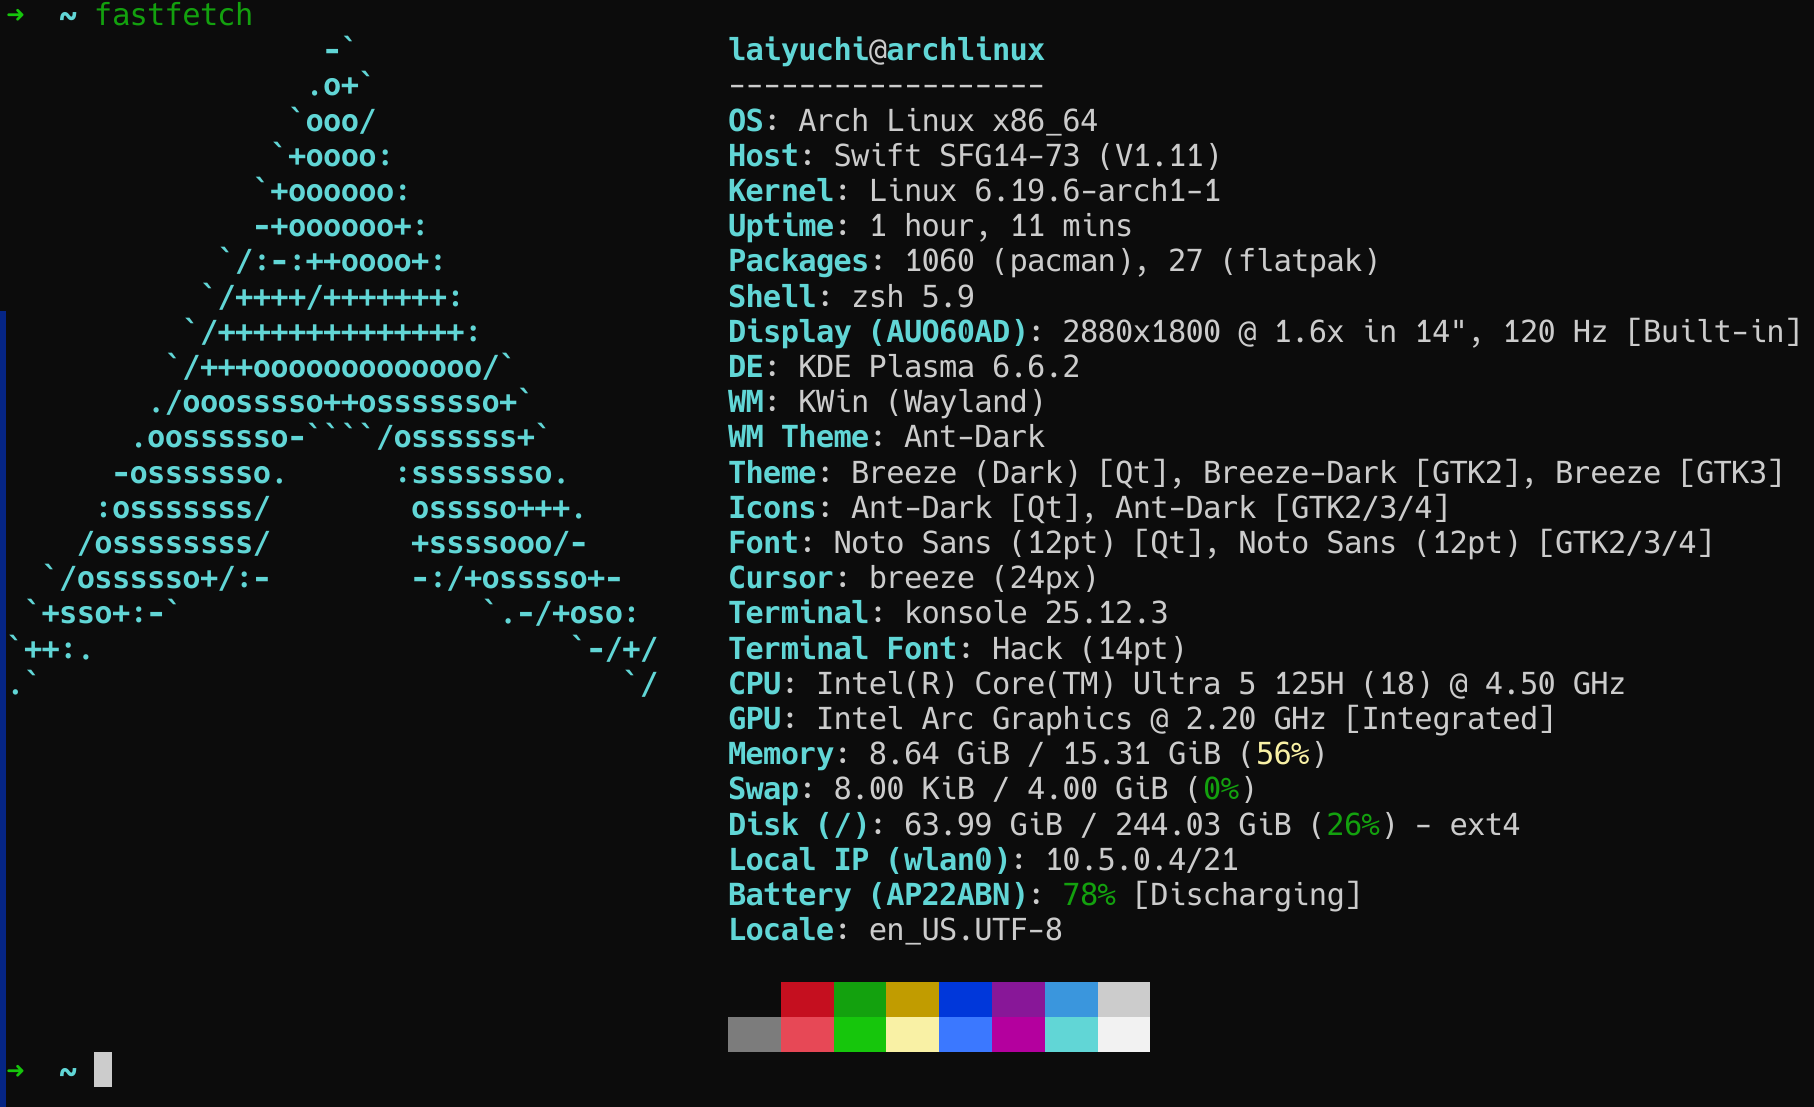
\includegraphics[width=0.9\linewidth]{image/Arch_fastfetch.png} 
   \caption{The result of \texttt{fastfetch} (It could be installed through \texttt{pacman -S fastfetch})}
\end{figure}
\subsection{Setup}
\noindent In all following implementations and tests, the multi-threading is \textbf{disabled} (see lines 1-5)

\inputminted[frame=lines,framesep=2mm,baselinestretch=1.2,fontsize=\footnotesize,linenos,breaklines]{bash}{code/setup.sh}
\begin{itemize}
    \item Line 1-5: Setup the environment for Intel oneMKL, OpenBLAS and CBLAS
    \item Line 7-14: Build the environment for AMD BLIS (according to the document of this \href{https://github.com/amd/blis}{repo})
    \item Line 16: How I compile my code and link cblas.h to BLIS implementation
    \item Line 18: How I compile my code and link cblas.h to Intel oneMKL implementation
    \item Line 20: How I compile my code and link cblas.h to openblas implementation
    \item Line 22: How I compile my code and link cblas.h to netlib/CBLAS implementation
    \item Line 24-28: Setting up the virtual environment for the installation of SciPy.
\end{itemize}
\section{Code}
\subsection{Steepest Descent Method}

\noindent Usage (after compilation): \texttt{./my\_steepest\_descent n}, where integer \texttt{n} is the size of the matrix. After running, it will writes A, x and b of the linear equation $Ax=b$ into the text file of same name.
\inputminted[frame=lines,framesep=2mm,baselinestretch=1.2,fontsize=\footnotesize,linenos,breaklines]{c}{code/my_steepest_descent.c}
\subsection{Correctness Checker}
\noindent Usage: \texttt{python solution\_checker.py}. After execution, the program will reads $A$ and $b$ from the text file generated previously, and then calculate the solution $x$ in $Ax=b$, print it out in the end.
\inputminted[frame=lines,framesep=2mm,baselinestretch=1.2,fontsize=\footnotesize,linenos,breaklines]{python}{code/solution_checker.py}
\section{Result}
\subsection{Correctness of my code}

\begin{figure}[H]
    \centering
    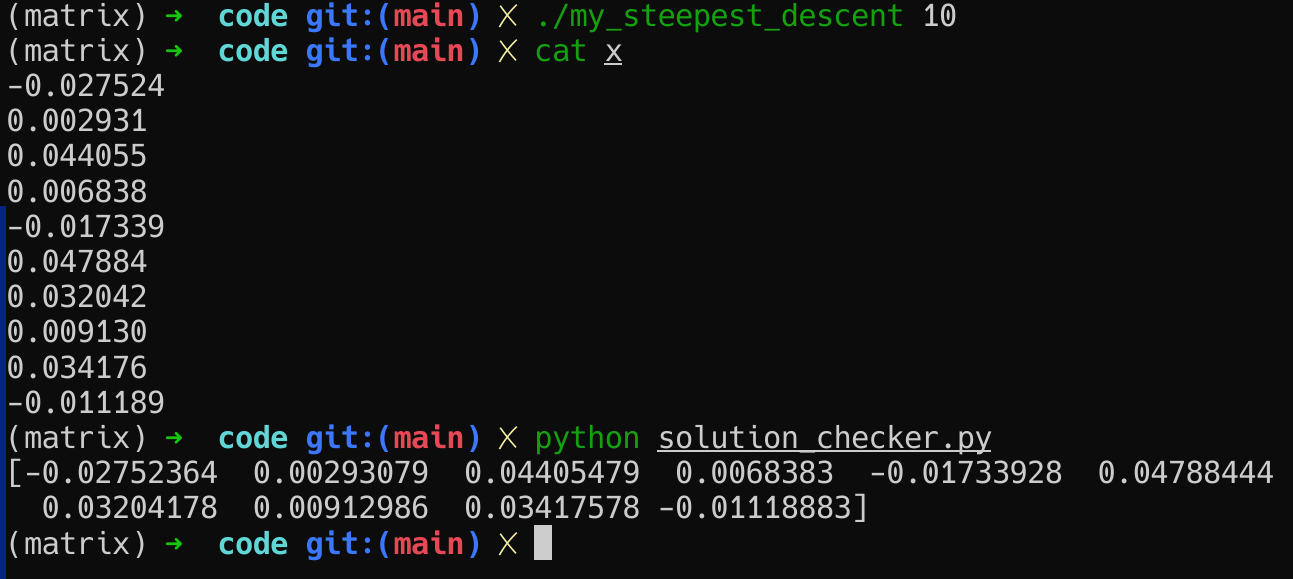
\includegraphics[width=0.6\linewidth]{image/correctness.png}
    \caption{Using the checker on $n=10$ case (openblas implementation, but other implementation is also correct), we can see our result is correct, align with the results from SciPy.}
\end{figure}
\subsection{Performance on different matrix sizes}
We use the built-in \texttt{time} command in linux to calculte the Real (Elapsed), User (user space) and Sys (kernel) time. The command is \texttt{time ./my\_steepest\_descent n}.
\begin{table}[H]
    \centering
    \vspace{0.5em}
    \begin{tabular}{clrrr}
        \toprule
        \textbf{Size ($N$)} & \textbf{Library} & \textbf{Real (s)} & \textbf{User (s)} & \textbf{Sys (s)} \\
        \midrule
        \multirow{4}{*}{100} 
        & Intel MKL & 0.19 & 0.03 & 0.07 \\
        & OpenBLAS & 0.06 & 0.01 & 0.04 \\
        & Netlib CBLAS & 0.01 & 0.01 & 0.00 \\
        & AMD BLIS & 0.05 & 0.01 & 0.04 \\
        \midrule
        \multirow{4}{*}{500} 
        & Intel MKL & 0.24 & 0.22 & 0.02 \\
        & OpenBLAS & 0.23 & 0.21 & 0.01 \\
        & Netlib CBLAS & 0.69 & 0.63 & 0.01 \\
        & AMD BLIS & 0.27 & 0.20 & 0.01 \\
        \midrule
        \multirow{4}{*}{1000} 
        & Intel MKL & 1.87 & 1.79 & 0.04 \\
        & OpenBLAS & 1.40 & 1.36 & 0.03 \\
        & Netlib CBLAS & 5.08 & 5.04 & 0.02 \\
        & AMD BLIS & 1.48 & 1.44 & 0.03 \\
        \midrule
        \multirow{4}{*}{4000} 
        & Intel MKL & 191.29 & 189.53 & 0.42 \\
        & OpenBLAS & 259.38 & 256.78 & 0.43 \\
        & Netlib CBLAS & 334.64 & 332.70 & 0.31 \\
        & AMD BLIS & 206.97 & 204.60 & 0.35 \\
        \bottomrule
    \end{tabular}
    \caption{Execution Time Comparison of BLAS Libraries for \texttt{my\_steepest\_descent}}
    \label{tab:blas_comparison}
\end{table}

We can see that the intel oneMKL and AMD blis performs much better than openblas and netlib/CBLAS when $n$ is large ($n=4000$). The implementation from netlib is the worst one with respect to execution time.
\section{Analysis}
In High-Performance Computing (HPC), the performance gap between Vendor-Optimized (Intel MKL, AMD AOCL), Optimized Open-Source (OpenBLAS, BLIS), and Reference Implementations (Netlib CBLAS) is driven by three primary architectural optimizations.

\subsection*{1. The Memory Wall \& Cache Blocking}
The primary bottleneck in dense linear algebra is moving data from main memory to the CPU. Matrix multiplication requires $\mathcal{O}(n^3)$ operations on only $\mathcal{O}(n^2)$ data. High-performance libraries solve this using \textbf{multi-level cache blocking}. They slice matrices into specific blocks sized perfectly to fit into the processor's L1, L2, and L3 caches, as well as the Translation Lookaside Buffer (TLB). Netlib fails here because it uses naive nested loops, causing devastating cache misses.
\begin{itemize}[noitemsep, topsep=2pt]
    \item \textbf{Reference:} \href{https://doi.org/10.1145/1356052.1356053}{\textit{Anatomy of High-Performance Matrix Multiplication}} by Kazushige Goto and Robert van de Geijn (2008). This paper defines the ``Goto Algorithm,'' which forms the foundational cache-blocking strategy for GotoBLAS and OpenBLAS.
\end{itemize}

\subsection*{2. Hand-Tuned Assembly \& SIMD Vectorization}
Modern CPUs feature Single Instruction, Multiple Data (SIMD) units (e.g., AVX-512, NEON) that process multiple floating-point numbers per clock cycle. To maximize throughput, the innermost loops (``micro-kernels'') cannot be written in standard C; they must be written in hand-tuned assembly. Intel MKL and AMD BLIS leverage proprietary knowledge of their silicon to write cycle-perfect assembly. Netlib relies purely on compiler auto-vectorization, which is highly inefficient for complex matrix workloads.
\begin{itemize}[noitemsep, topsep=2pt]
    \item \textbf{Reference:} \href{https://doi.org/10.1145/2764454}{\textit{BLIS: A Framework for Rapidly Instantiating BLAS Functionality}} by Field G. Van Zee and Robert A. van de Geijn (2015). This paper explicitly details how BLIS isolates hardware-specific assembly into a tiny micro-kernel to achieve MKL-like performance.
\end{itemize}

\subsection*{3. Smart Multithreading and NUMA Awareness}
Optimized libraries are explicitly designed for modern multi-core and Non-Uniform Memory Access (NUMA) architectures. Intel MKL binds threads strictly to physical cores (avoiding hyperthreading bottlenecks) and ensures memory is processed by the physically closest CPU socket. Netlib is strictly single-threaded and lacks parallel execution capabilities natively.
\begin{itemize}[noitemsep, topsep=2pt]
    \item \textbf{Reference:} \href{https://netlib.org/scalapack/slug/node158.html}{\textit{ScaLAPACK Users' Guide: Poor Performance (Netlib)}}. The official documentation explicitly warns: ``Although a reference implementation... is available from the blas directory on netlib, these routines are not expected to perform as well as a specially tuned implementation... Users are urged to determine whether such an implementation of the BLAS exists for their platform.''
\end{itemize}


\end{document}